\documentclass[landscape, a4paper]{article}
\usepackage[top=0cm, bottom=0cm, left=0cm, right=0cm]{geometry}
\usepackage{tikz}
\usepackage{hyperref}
\usepackage{marvosym}
\usepackage[utf8]{inputenc}
\usetikzlibrary{patterns}
\usetikzlibrary{shapes,arrows}
\usetikzlibrary{decorations.pathreplacing, positioning}
\definecolor{anti-flashwhite}{rgb}{0.95, 0.95, 0.96}


\begin{document}
\noindent
  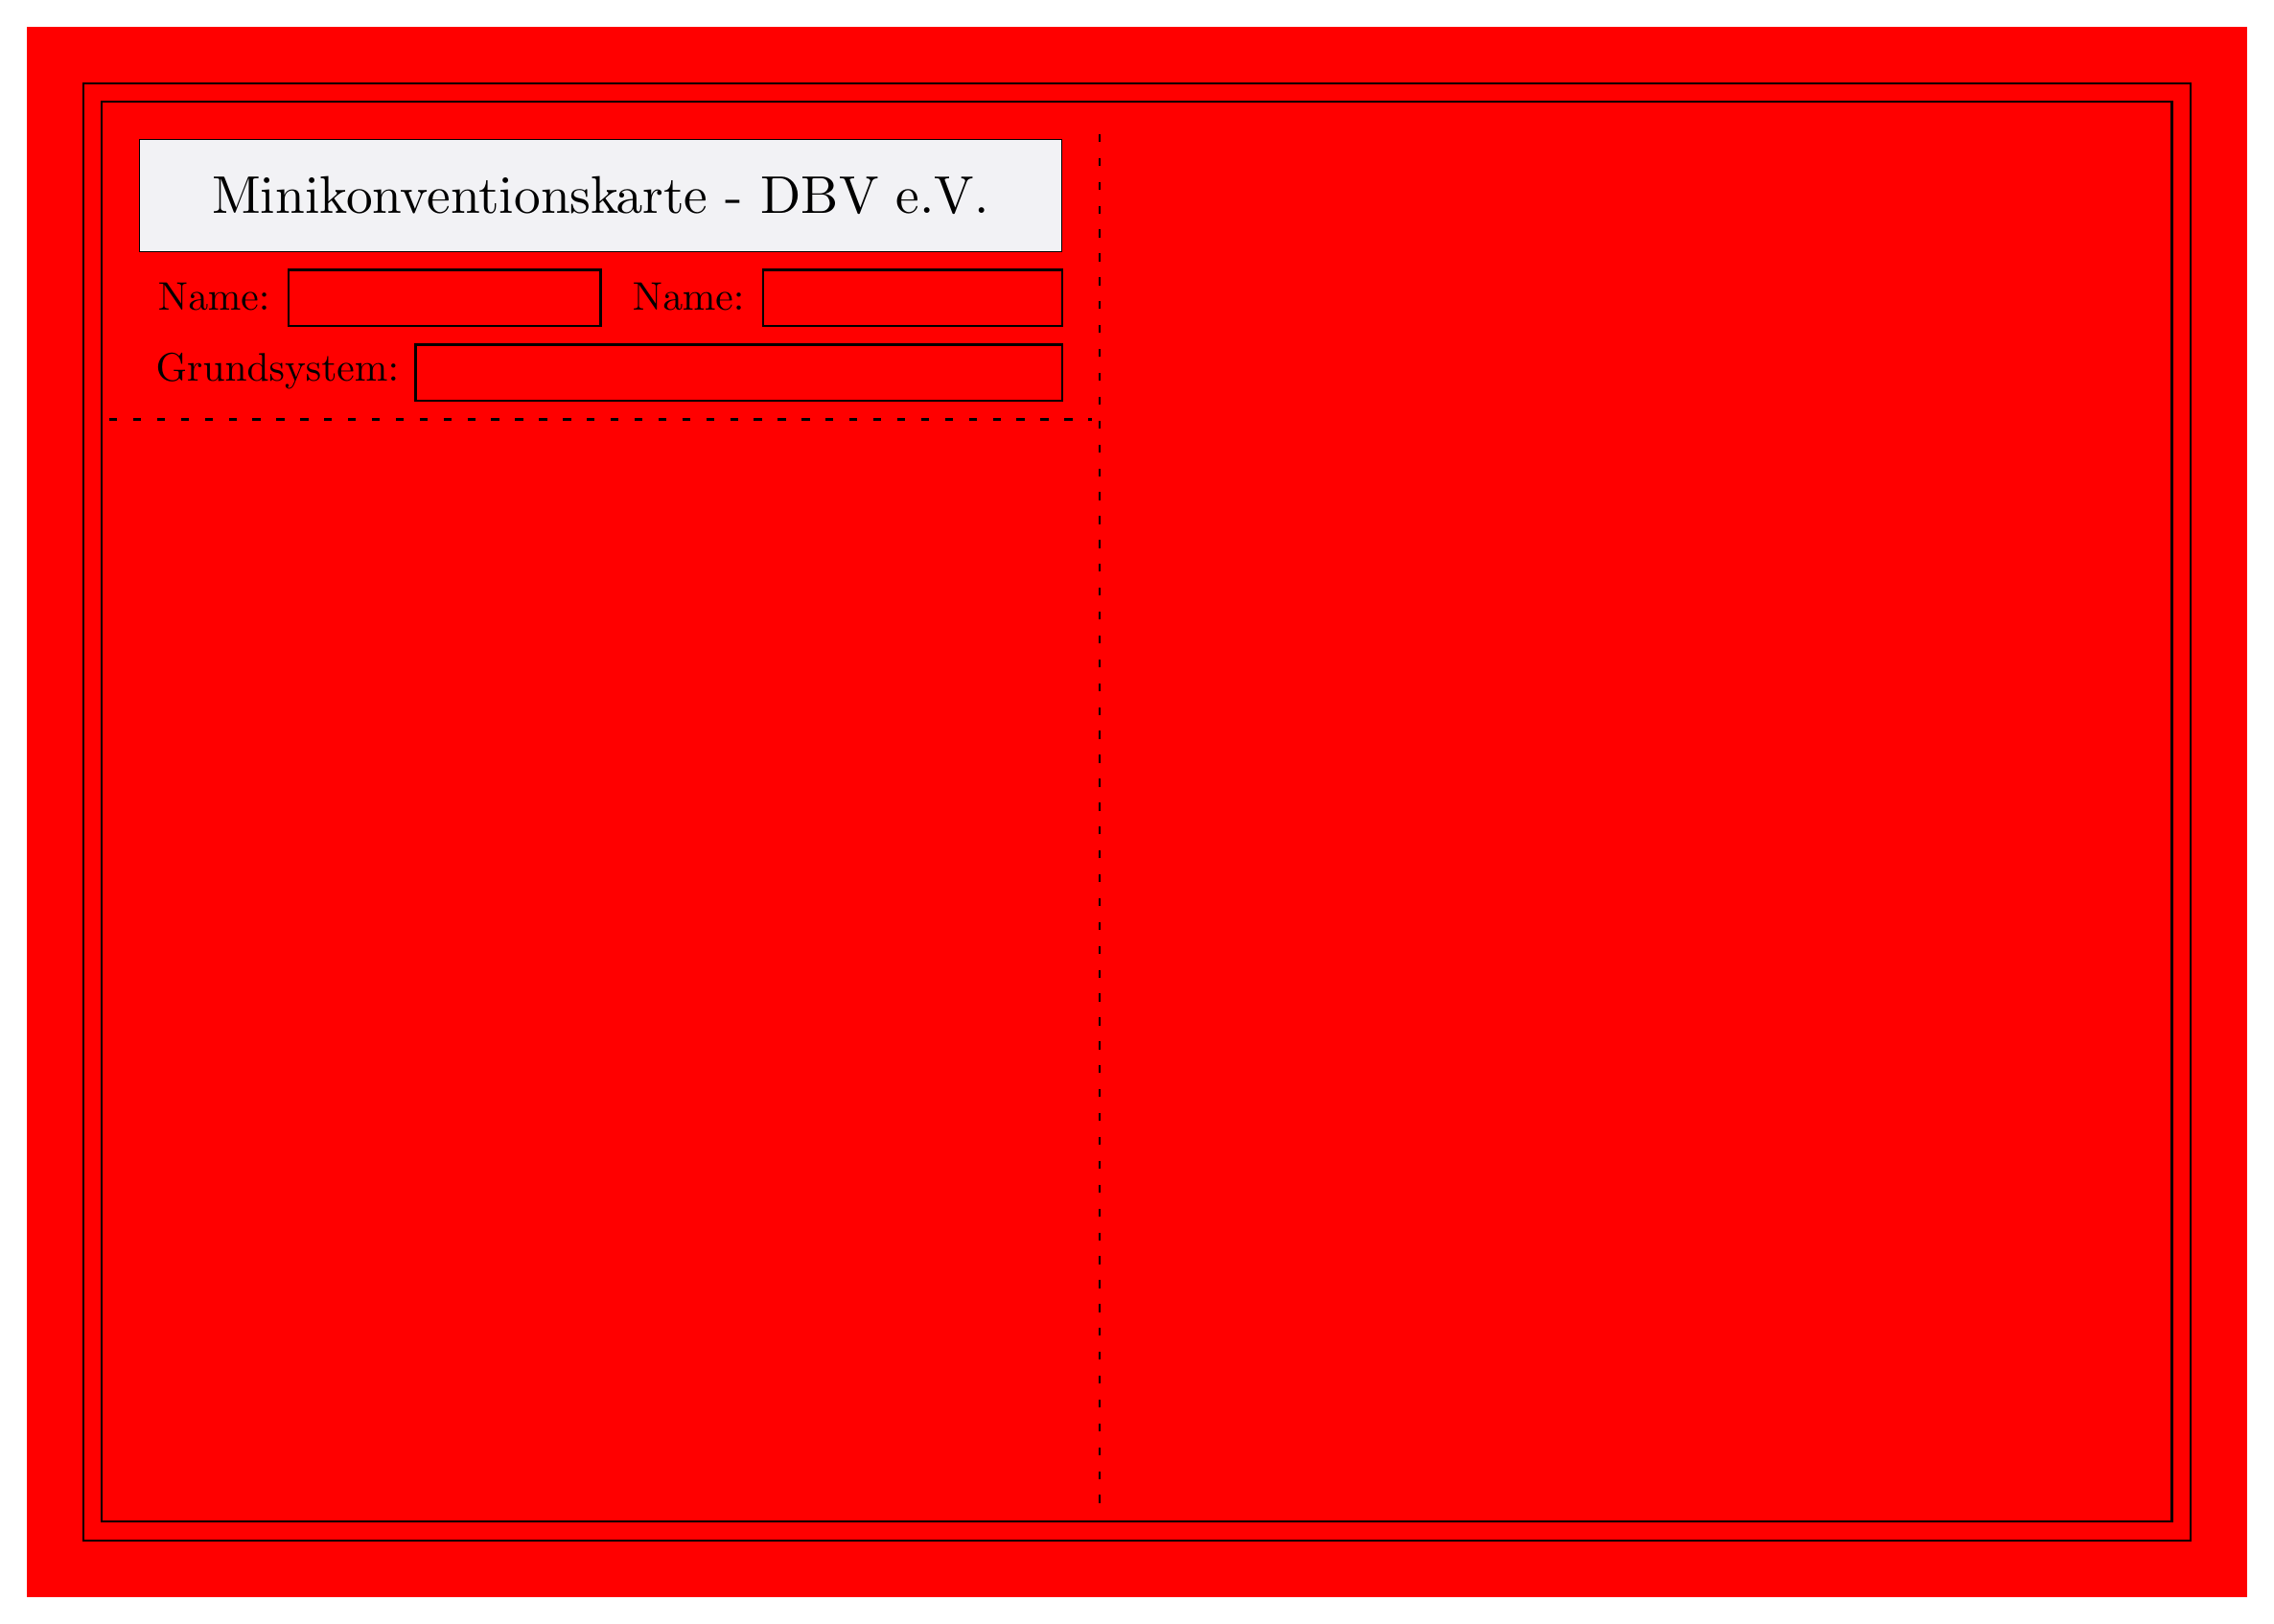
\begin{tikzpicture}[scale=0.99]
    % Background
    \draw[fill=white, color=red!!20] (0,0) -- (0,21) -- (29.7, 21) -- (29.7, 0) -- cycle;

    \foreach \x in {0, 0.25}
      \draw[thick] (1 - \x, 1 - \x) -- (28.7 + \x, 1 - \x) -- (28.7 + \x, 20 + \x) -- (1 - \x, 20 + \x) -- cycle;

    \draw[thick, loosely dashed] (14.35, 1.25) -- (14.35, 19.75);

    \draw[fill=anti-flashwhite] (1.5, 19.5) -- (13.85, 19.5) -- (13.85, 18) -- (1.5, 18) -- cycle;

    \node[very thick, align=center, scale=2] at (7.675, 18.75) {Minikonventionskarte - DBV e.V.};

    \draw[thick] (7.675, 17.75) -- (3.5, 17.75) -- (3.5, 17) -- (7.675, 17) -- cycle;

    \draw[thick] (13.85, 17.75) -- (9.85, 17.75) -- (9.85, 17) -- (13.85, 17) -- cycle;

    \node[thick, align=center, scale=1.5] at (2.5, 17.4) {Name:};
    \node[thick, align=center, scale=1.5] at (8.85, 17.4) {Name:};


    \draw[thick] (5.2, 16.75) -- (13.85, 16.75) -- (13.85, 16) -- (5.2, 16) -- cycle;

    \node[thick, align=center, scale=1.5] at (3.35, 16.4) {Grundsystem:};

    \draw[thick, loosely dashed] (1.1, 15.75) -- (14.25, 15.75);

  \end{tikzpicture}
\end{document}
